% !TEX TS-program = xelatex
% !TEX encoding = UTF-8 Unicode
% !Mode:: "TeX:UTF-8"

%This file contains the LaTeX code of my laboratory report for my Database course.
%Author: 黄佳妮/Jiani Huang <17302010063@fudan.edu.cn>
%Author: 刘佳兴/Jiaxing Liu <17302010049@fudan.edu.cn>


% This is a simple template for a LaTeX document using the "article" class.
% See "book", "report", "letter" for other types of document.
\documentclass[12pt]{article} % use larger type; default would be 10pt

\usepackage[utf8]{inputenc} % set input encoding (not needed with XeLaTeX)

%%% Examples of Article customizations
% These packages are optional, depending whether you want the features they provide.
% See the LaTeX Companion or other references for full information.

%%% PAGE DIMENSIONS
\usepackage[top=1.05in, bottom=0.95in, left=0.90in, right=1.10in]{geometry}
%\usepackage{geometry} % to change the page dimensions
\geometry{a4paper} % or letterpaper (US) or a5paper or....
% \geometry{margin=2in} % for example, change the margins to 2 inches all round
% \geometry{landscape} % set up the page for landscape
%   read geometry.pdf for detailed page layout information

\usepackage{graphicx} % support the \includegraphics command and options

% \usepackage[parfill]{parskip} % Activate to begin paragraphs with an empty line rather than an indent

%%% PACKAGES
\usepackage{booktabs} % for much better looking tables
\usepackage{array} % for better arrays (eg matrices) in maths
\usepackage{paralist} % very flexible & customisable lists (eg. enumerate/itemize, etc.)
\usepackage{verbatim} % adds environment for commenting out blocks of text & for better verbatim
%\usepackage{subfig} % make it possible to include more than one captioned figure/table in a single float
% These packages are all incorporated in the memoir class to one degree or another...


%%% HEADERS & FOOTERS
\usepackage{fancyhdr} % This should be set AFTER setting up the page geometry
\pagestyle{fancy} % options: empty , plain , fancy
%\renewcommand{\headrulewidth}{0pt} % customise the layout...
\lhead{}\chead{}\rhead{}
\lfoot{}\cfoot{\thepage}\rfoot{}

%%% SECTION TITLE APPEARANCE
\usepackage{sectsty}
\allsectionsfont{\sffamily\mdseries\upshape} % (See the fntguide.pdf for font help)
% (This matches ConTeXt defaults)

%%% ToC (table of contents) APPEARANCE
\usepackage[nottoc,notlof,notlot]{tocbibind} % Put the bibliography in the ToC
\usepackage[titles,subfigure]{tocloft} % Alter the style of the Table of Contents
\renewcommand{\cftsecfont}{\rmfamily \mdseries \upshape}
\renewcommand{\cftsecpagefont}{\rmfamily \mdseries \upshape} % No bold!
\usepackage{titletoc}
\titlecontents{section}
              [1.5cm]
              {\bf \large}%
              {\contentslabel{1.8em}}%
              {}%
              {\titlerule*[0.5pc]{$\cdot$}\contentspage\hspace*{0.6cm}}%
		   [\vspace{0.5em}]
\titlecontents{subsection}
              [1.8cm]
              {\normalsize}%
              {\contentslabel{2.0em}}%
              {}%
              {\titlerule*[0.5pc]{$\cdot$}\contentspage\hspace*{0.6cm}}%
		   [\vspace{0.4em}]
\titlecontents{subsubsection}
              [2.1cm]
              {\small}%
              {\contentslabel{2.5em}}%
              {}%
              {\titlerule*[0.5pc]{$\cdot$}\contentspage\hspace*{0.6cm}}%
		   [\vspace{0.4em}]

\usepackage[UTF8]{ctex}
\usepackage{fancyhdr}
\usepackage{enumerate}
\usepackage{indentfirst}
\usepackage{extramarks}
\usepackage{titling}
\usepackage{listings}
\usepackage{xcolor}
\usepackage{fontspec}
\usepackage{float} 
\usepackage{subfigure}
\usepackage[CJKbookmarks=true,colorlinks,linkcolor=black]{hyperref}
\usepackage{amsmath}
\usepackage{amssymb}
\usepackage{ulem}
\usepackage{stackengine}
\let\tuwave\uwave
\newcommand\buline[1]{\raisebox{-3pt}{\uline{\raisebox{2pt}{#1}}}}

\definecolor{mygreen}{rgb}{0,0.6,0}  
\definecolor{mygray}{rgb}{0.9,0.9,0.9}  
\definecolor{mymauve}{rgb}{0.58,0,0.82}  
\definecolor{dkgreen}{rgb}{0,0.6,0}
\definecolor{ltgray}{rgb}{0.5,0.5,0.5}
  
\lstset{%
  	backgroundcolor=\color{mygray},
  	basicstyle={
		\footnotesize
		\fontspec{Consolas}
	},
  	breakatwhitespace=false,
  	breaklines=true,
  	captionpos=bl,
  	commentstyle={
		\color{mygray}
		\fontspec{Consolas Italic}
	},
  	deletekeywords={identity,date,year,...},
  	escapeinside={\%*}{*)},
  	extendedchars=true,
  	%frame=single,
  	keepspaces=true,
  	keywordstyle={
		\color{blue}
		\fontspec{Consolas Bold}
	},
  	language=SQL,
  	morekeywords={*,modify,MODIFY,...},
  	numbers=none,
  	numbersep=5pt,
  	numberstyle=\tinyy\color{mygray},
  	rulecolor=\color{black},
  	showspaces=false,
  	showstringspaces=false, 
  	showtabs=false,
  	stepnumber=1,
  	tabsize=4,
	stringstyle=\color{blue},
  	title=\lstname,
	belowcaptionskip=0em,
    	belowskip=0em,
}

\newfontfamily\myfont{Consolas}


%%% END Article customizations

%%% The "real" document content comes below...

%\title{\textbf{Digital Logic and Computer Design Report}}
\title{\textbf{选课系统项目需求文档}}
\author{黄佳妮 17302010063 \\刘佳兴 17302010049}
%\date{} % Activate to display a given date or no date (if empty),
         % otherwise the current date is printed 

\begin{document}
\begin{sloppypar}
\maketitle

\pagestyle{fancy}
\lhead{\textbf{{\thetitle}}}
\rhead{\textbf{\nouppercase{\firstleftmark}}}
\cfoot{\thepage}

\thispagestyle{empty}
\tableofcontents
\thispagestyle{empty}
\clearpage

\setcounter{page}{1}

\section{项目概述}

我们将以复旦选课系统为例,完成一个简化版选课系统,其中体现数据库设计的思想。

\subsection{项目背景}
选课系统的实现分为客户端和服务器端两部分。而数据库设计的增删改查部分将在服务器部分体现。

\subsection{项目功能概述}

本项目的大致系统功能如下:(详细版如限制检查等请查看功能需求部分)

\begin{table}[h]
\begin{tabular}{ll}
{\bf 教师信息管理}   & 教师信息自动导入数据库 \\
{\bf 学生信息管理} & 学生信息自动导入数据库 \\
{\bf 课程开设}   & 课程信息的自动导入数据库 \\
{\bf 登陆/登出系统1}   & 学生/老师使用学/工号可登陆系统。 \\
{\bf 登陆/登出系统2}   & root管理员可增删改查所有信息。 \\
{\bf 学生选/退课}   & 学生可以查看目前课程的开设及选课情况,且在任意时间节点选/退课。 \\
{\bf 选课事务申请1}   & 学生对于选课人数已满的课程可以提交选课申请并查看申请状态。 \\
{\bf 选课事务申请2}   & 老师可以审核选课事务申请。 \\
{\bf 登分1}   & 管理员自动/手动录入学生课程成绩。 \\  
{\bf 登分2}   & 学生查看成绩。 \\ 
{\bf 登分3}   & 老师通过导入excel的方式自动登分。 \\ 
\end{tabular}
\end{table}


%插入泳道图 用况图

\subsubsection{教师信息管理}
系统管理员将教师信息(学院、工号、姓名等)手动或自动导入教师数据库中

\subsubsection{学生信息管理}
系统管理员将学生信息(学院、学号、姓名、专业等)手动或自动导入数据库

\subsubsection{课程开设}
课程信息(课程代码、课程名称、学分、任课老师、时间、地点、课时、人数/最大人数、考试时间等)的自动导入数据库

\subsubsection{登陆/登出系统}
学生/老师使用学/工号可登陆系统,查看其对应权限下的信息;root管理员可增删改查所有信息。

\subsubsection{学生选/退课}
学生可以查看目前课程的开设及选课情况,且在任意时间节点选/退课。

\subsubsection{选课事务申请}
学生对于选课人数已满的课程可以提交选课申请并查看申请状态;老师可以审核选课事务申请。

\subsubsection{登分}
管理员自动/手动录入学生课程成绩;学生查看成绩;老师通过导入excel的方式自动登分。




\subsection{项目模块划分}
 

\subsection{项目用户特征}
\subsubsection{教师}
教师可以使用工号登陆系统,查看教师权限下的所有信息(课程花名册/管理选课事务申请)。除此以外,教师还可以将对应课程的学生成绩导入系统。
\subsubsection{学生}
学生可以使用学号登陆系统,查看学生权限下的所有信息(成绩/课程表/选课申请/课程的开设及选课情况)。并且,学生可以对选课人数已达上限但仍没有超过教室容量的课程进行选课申请。
\subsubsection{管理员/院系}
院系(信息办工作人员)可以拿到root管理员权限,并进行数据的自动导入,可以查看所有信息并手动/自动增加条目,可以通过课程代码删除课程。


\subsection{开发框架}

\begin{table}[h]
\begin{tabular}{ll}
{\bf 开发语言}   & JavaScript / HTML / CSS / Python / SQLite \\
{\bf 浏览器环境} & Chrome / Safari \\
{\bf 第三方库}   & Ant-Design / Django                             
\end{tabular}
\end{table}








\section{细化功能需求}
\begin{itemize}
    \item 教师信息、学生信息、课程信息自动导入数据库,且需要检查相应冲突(时间/地点/任课老师等)。
    \item 课程:一周内可能多次开课、可能通过论文考试、课时按照小时为单位。
    \item 共有三类权限人员:学生、老师、管理员(院系)。
    \item 三类权限人员使用各自登陆方式登陆系统后,可查看其各自权限下的所有信息。
    \item 学生权限:使用学号和密码登陆,查看成绩/课程表/选课申请。
    \item 老师权限:使用工号和密码登陆,查看课程花名册/管理选课事务申请。
    \item 管理员权限:使用root和密码登陆,查看所有信息并且自动导入/课程删除操作。
    \item 学生的选课和退课操作可以在任何时间进行,先到先得。
    \item 选课需要系统进行冲突检查(考试和上课)。
    \item 进行数据的本地化操作 或 在启动系统时有默认内部数据。
    \item 当且仅当课程的选课人数到达上限,学生可以填写选课申请。
    \item 相应课程的教师负责处理选课申请,可以选择通过或不通过。
    \item 当学生所选课程的选课人数超出教室可容纳人数时,系统自动驳回尚未处理的选课申请,关闭该课程的申请窗口。
    \item 学生可以查看选课申请状态。
    \item 学生不能申请已选课程。
    \item 考试时间为特定周到第18周,和上课时间不会冲突。
    \item 系统自动/手动导入学生课程成绩
    \item 学生可以查看该学期成绩单和总绩点
    \item 教师可以通过excel方式登分。
\end{itemize}


\begin{figure}[h]
    \centering
    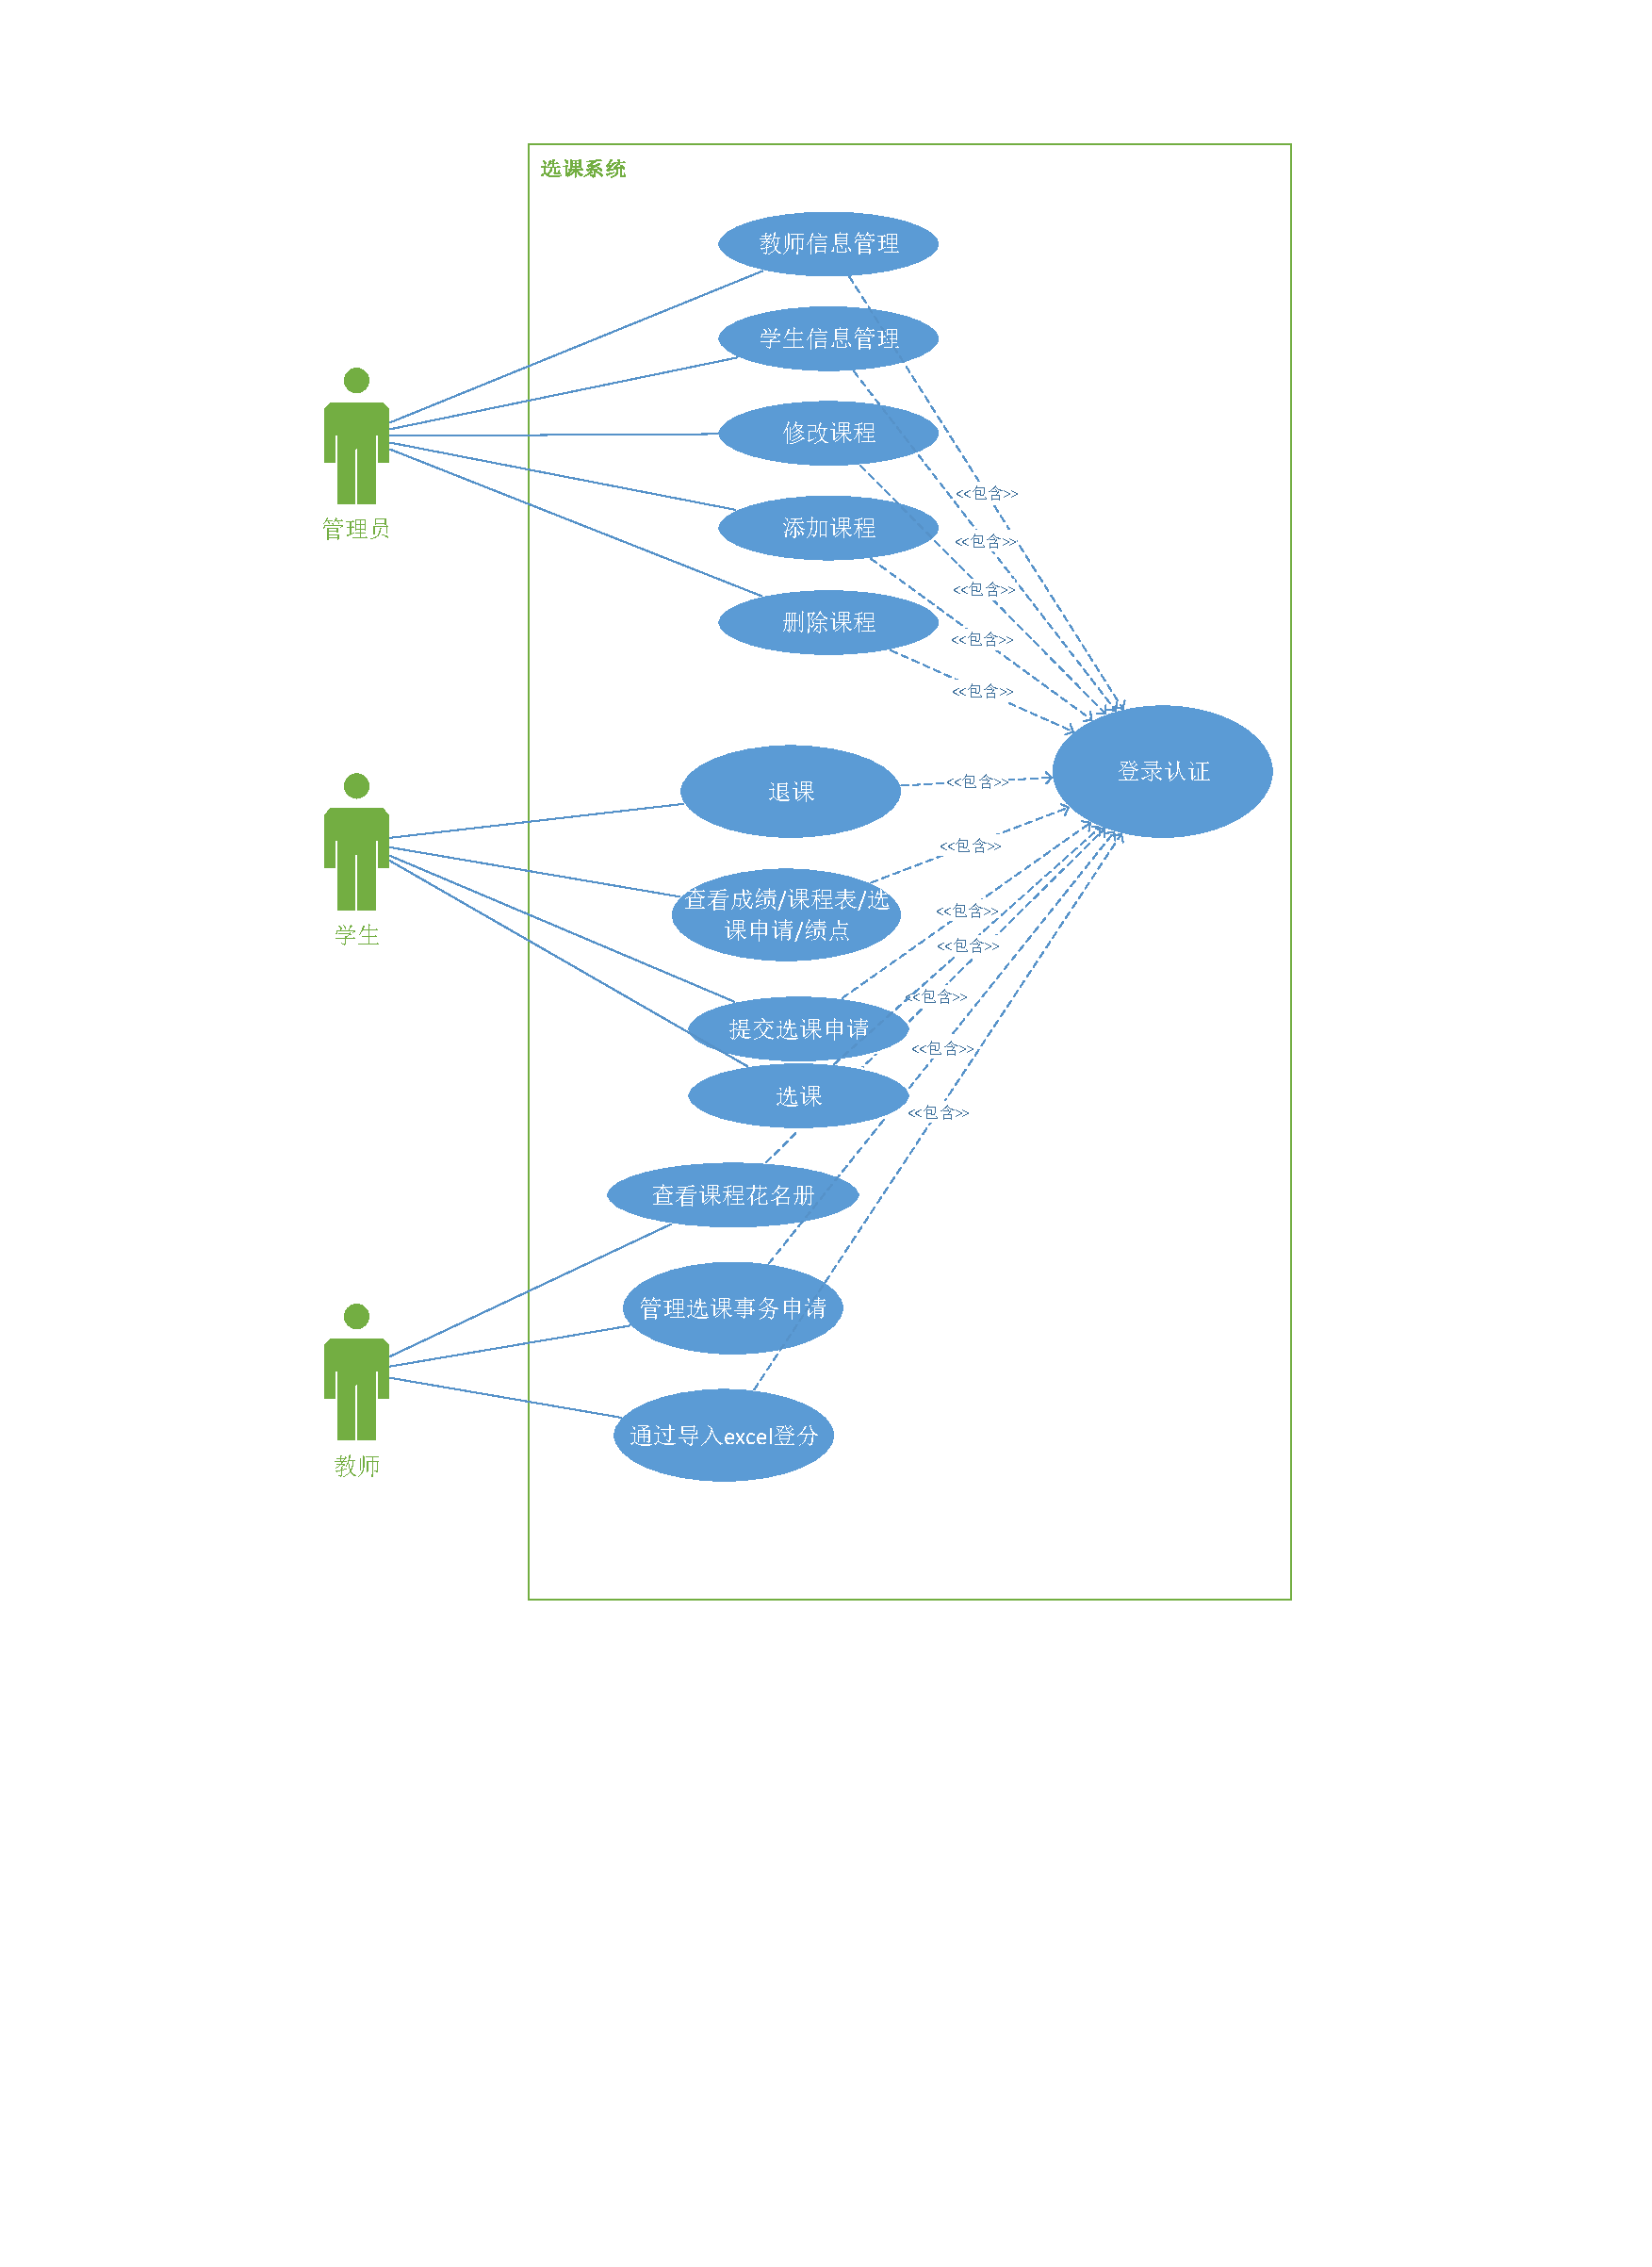
\includegraphics[width=0.8\textwidth]{assets/courseTakingusercase.pdf}
    \end{figure}

\subsection{限制检查}
\subsubsection{开设课程}
系统管理员导入或添加课程时,系统需要检查课程的相关信息是否存在冲突。检查包括但不限于:同一任课教师在多门课程的任课时间是否存在冲突;多门课程在时空上是否存在冲突;每一门课程涉及的时间和教室是否可用。系统发现冲突需要暂停执行并给出相应提示。
\subsubsection{选修课程}
学生选择课程时,系统需要检查选课的相关信息是否存在冲突。检查包括但不限于:同一学生选择的多门课程的上课时间是否存在冲突;同一学生选择的多门课程的考试时间是否存在冲突。系统发现冲突需要暂停执行并给出相应提示。
\subsubsection{选课申请}
当且仅当课程的选课人数到达上限,学生可以填写选课申请,否则,系统自动驳回。并且学生不能申请选已退课程。当学生所选课程的选课人数超出教室可容纳人数时,系统自动驳回尚未处理的选课申请,关闭该课程的申请窗口。
\subsection{测试需求}

\begin{itemize}
    \item 自动导入课程功能:在初始数据中出现冲突数据,并抛出相关提示。
    \item 选退课功能:在初始数据中出现冲突数据,并抛出相关提示。
\end{itemize}





\end{sloppypar}
\end{document}
